\documentclass[pdflatex,compress,mathserif]{beamer}

%\usetheme[dark,framenumber,totalframenumber]{ElektroITK}
\usetheme[darktitle,framenumber,totalframenumber]{ElektroITK}

\usepackage[utf8]{inputenc}
\usepackage[T1]{fontenc}
\usepackage{lmodern}
\usepackage[english]{babel}
\usepackage{amsmath}
\usepackage{amsfonts}
\usepackage{amssymb}
\usepackage{graphicx}
\usepackage{multicol}
\usepackage{lipsum}
\usepackage{framed}
\usepackage{minted}

\definecolor{LightGray}{gray}{0.95}

\usefonttheme[onlymath]{serif}

\newcommand*{\Scale}[2][4]{\scalebox{#1}{$#2$}}%

\setbeamertemplate{caption}[numbered]

\title{Digital Signal Processing}
\subtitle{Realization}

\author{Mifta Nur Farid}
\date{Sept. $\text{4}^\text{st}$, 2023}

\begin{document}

\maketitle

\begin{frame}{Difference Equation and\\Digital Filtering}
	\begin{figure}
		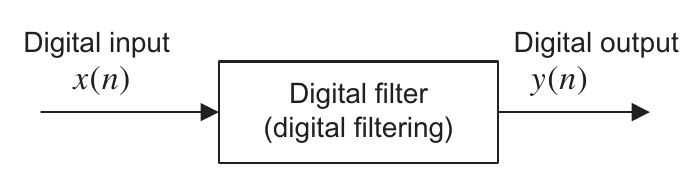
\includegraphics[width=0.7\linewidth]{./img/img01.png}
	\end{figure}
	\begin{itemize}
		\item Expressed by difference equation:
		\begin{align*}
			y(n) = &~ b_0 x(n) + b_1 x(n-1) + \cdots +b_Mx(n-M)\\
				   & -a_1y(n-1) - \cdots - a_ny(n-N)
		\end{align*}
		or
		\begin{align*}
			y(n) = \sum_{i=0}^{M} b_i x(n-i) - \sum_{j=1}^{N} a_j y(n-j)
		\end{align*}
	\end{itemize}
\end{frame}

\begin{frame}{Difference Equation and\\Transfer Function}
	\begin{itemize}
		\item Difference Equation:
		\begin{align*}
			y(n) = &~ b_0 x(n) + b_1 x(n-1) + \cdots +b_Mx(n-M)\\
				   & -a_1y(n-1) - \cdots - a_ny(n-N)
		\end{align*}
		\item Expressed in $z$-domain
		\begin{align*}
			Y(z) = &~ b_0 X(z) + b_1 X(z)z^{-1} + \cdots + b_M X(z)z^{-M}\\
				   & -a_1Y(z)z^{-1} - \cdots - a_n Y(z)z^{-N}
		\end{align*}
		\item Expressed by transfer function in $z$-domain
		\begin{align*}
			H(z) = \frac{Y(z)}{X(z)} = \frac{b_0 + b_1z^{-1} + \cdots + b_M z^{-M}}{1 + a_1z^{-1} + \cdots + a_n z^{-N}} = \frac{B(z)}{A(z)}
		\end{align*}
	\end{itemize}
\end{frame}

\begin{frame}{Difference Equation and\\Transfer Function}
	\begin{itemize}
		\item Difference Equation:
		\begin{align*}
			y(n) = &~ b_0 x(n) + b_1 x(n-1) + \cdots +b_Mx(n-M)\\
				   & -a_1y(n-1) - \cdots - a_ny(n-N)
		\end{align*}
		\item Expressed in $z$-domain
		\begin{align*}
			Y(z) = &~ b_0 X(z) + b_1 X(z)z^{-1} + \cdots + b_M X(z)z^{-M}\\
				   & -a_1Y(z)z^{-1} - \cdots - a_n Y(z)z^{-N}
		\end{align*}
	\end{itemize}
\end{frame}

\begin{frame}{Difference Equation and\\Transfer Function}
	\begin{itemize}
		\item Expressed by transfer function in $z$-domain
		\begin{align*}
			H(z) = \frac{Y(z)}{X(z)} = \frac{b_0 + b_1z^{-1} + \cdots + b_M z^{-M}}{1 + a_1z^{-1} + \cdots + a_n z^{-N}} = \frac{B(z)}{A(z)}
		\end{align*}
	\end{itemize}
	\begin{figure}
		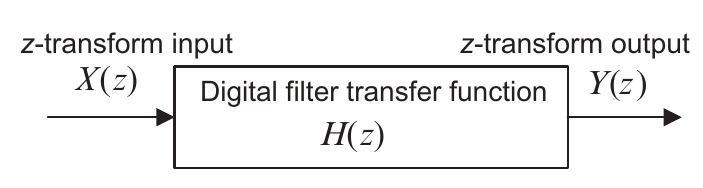
\includegraphics[width=0.7\linewidth]{./img/img02.png}
	\end{figure}
\end{frame}

\begin{frame}{Realization of Digital Filter}
	\begin{itemize}
		\item Digital filters described by the transfer function $H(z)$ may be generally realized into the following forms:
		\begin{enumerate}
			\item direct-form I
			\item direct-form II
			\item cascade
			\item parallel
		\end{enumerate}
	\end{itemize}
\end{frame}

\begin{frame}{Direct-Form I Realization}
	\begin{itemize}
		\item Transfer function in $z$-domain
		\begin{align*}
			H(z) = \frac{Y(z)}{X(z)} = \frac{b_0 + b_1z^{-1} + \cdots + b_M z^{-M}}{1 + a_1z^{-1} + \cdots + a_n z^{-N}} = \frac{B(z)}{A(z)}
		\end{align*}
		\item change to:
		\begin{align*}
			Y(z) = &~ b_0 X(z) + b_1 X(z)z^{-1} + \cdots + b_M X(z)z^{-M}\\
				   & -a_1Y(z)z^{-1} - \cdots - a_n Y(z)z^{-N}
		\end{align*}
		\item inverse $z$-transform, get difference equation:
		\begin{align*}
			y(n) = &~ b_0 x(n) + b_1 x(n-1) + \cdots +b_Mx(n-M)\\
				   & -a_1y(n-1) - \cdots - a_ny(n-N)
		\end{align*}
	\end{itemize}
\end{frame}

\begin{frame}{Direct-Form I Realization}
		\begin{figure}
      \centering
			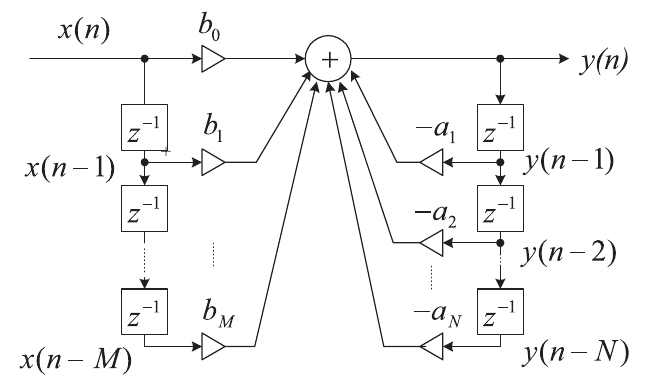
\includegraphics[width=\linewidth]{./img/img03.png}
		\end{figure}
\end{frame}

\begin{frame}{Direct-Form I Realization}
  \textbf{Example:}
  \begin{itemize}
    \item Given a second-order transfer function $$ H(z) = \frac{0.5(1-z^{-2})}{1 + 1.3z^{-1} + 0.36 z^{-2}} $$ perform the filter realizations and write difference equations using Direct-form I.
  \end{itemize}
\end{frame}

\begin{frame}{Direct-Form II Realization}
	\begin{itemize}
		\item Express transfer function with $N = M$ as:
		\begin{align*}
      Y(z) &= H(z) X(z) = \frac{B(z)}{A(z)} X(z) = B(z)\left( \frac{X(z)}{A(z)} \right) \\
      &= (b_0 + b_1 z^{-1} + \cdots + b_M z^{-M}) \left( \frac{X(z)}{1 + a_1 z^{-1} + \cdots + a_M z^{-M}} \right) \\
      &= (b_0 + b_1 z^{-1} + \cdots + b_M z^{-M}) W(z) \\
      &= b_0 W(z) + b_1 W(z) z^{-1} + \cdots + b_M W(z) z^{-M}
    \end{align*}
    \item inverse $z$-transform:
    \begin{align*}
      w(n) &= x(n) - a_1 w(n-1) - a_2 w(n-2) - \cdots - a_M w(n-M) \\
      y(n) &= b_0 w(n) + b_1 w(n-1) + \cdots + b_M w(n-M)
    \end{align*}
	\end{itemize}
\end{frame}

\begin{frame}{Direct-Form II Realization}
    \begin{figure}
      \centering
			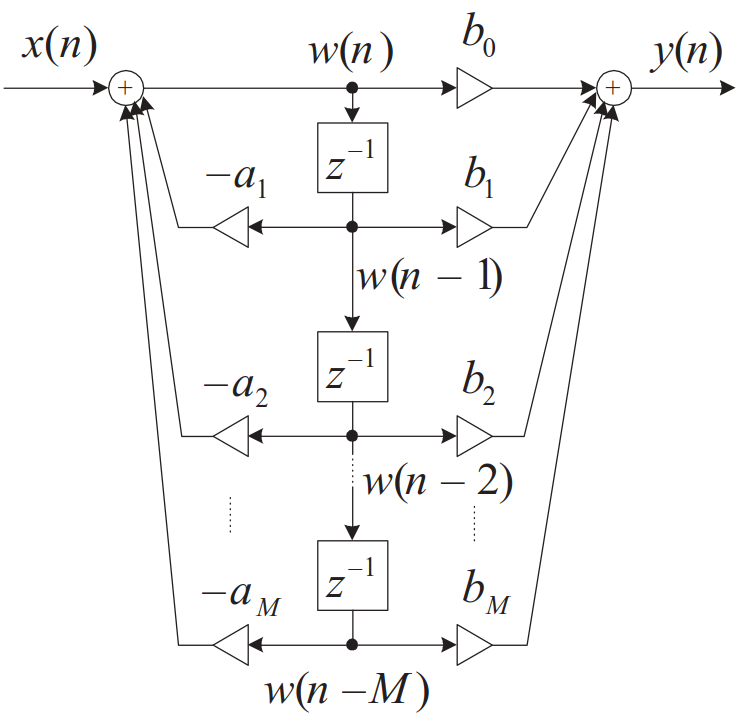
\includegraphics[width=0.6\linewidth]{./img/img04.png}
		\end{figure}
\end{frame}

\begin{frame}{Direct-Form II Realization}
  \textbf{Example:}
  \begin{itemize}
    \item Given a second-order transfer function $$ H(z) = \frac{0.5(1-z^{-2})}{1 + 1.3z^{-1} + 0.36 z^{-2}} $$ perform the filter realizations and write difference equations using Direct-form II.
  \end{itemize}
\end{frame}

\begin{frame}{Cascade (Series) Realization}
  \begin{itemize}
    \item cascade the factorized $H(z)$
    \begin{equation*}
      H(z) = H_1(z) \cdot H_2(z) \cdots H_k(z)
    \end{equation*}
    \item $H_k(z)$ is chosen to be the first-order transfer function
    \begin{align*}
      H_k(z) = \frac{b_{k0} + b_{k1}z^{-1}}{1 + a_{k1}z^{-1}}
    \end{align*}
    or second-order transfer function
    \begin{align*}
      H_k(z) = \frac{b_{k0} + b_{k1}z^{-1} + b_{k2}z^{-2}}{1 + a_{k1}z^{-1} + a_{k2}z^{-2}}
    \end{align*}
  \end{itemize}
\end{frame}

\begin{frame}{Cascade (Series) Realization}
  \begin{equation*}
    H(z) = H_1(z) \cdot H_2(z) \cdots H_k(z)
  \end{equation*}
  \begin{figure}
    \centering
    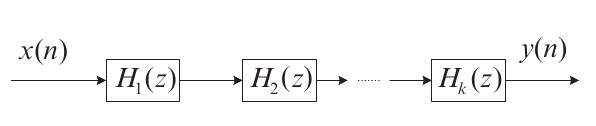
\includegraphics[width=0.8\linewidth]{./img/img05.png}
  \end{figure}
\end{frame}

\begin{frame}{Cascade (Series) Realization}
  \textbf{Example:}
  \begin{itemize}
    \item Given a second-order transfer function $$ H(z) = \frac{0.5(1-z^{-2})}{1 + 1.3z^{-1} + 0.36 z^{-2}} $$ perform the filter realizations and write difference equations using Cascade form via first-order sections
  \end{itemize}
\end{frame}

\begin{frame}{Parallel Realization}
  \begin{itemize}
    \item convert $H(z)$ into:
    \begin{equation*}
      H(z) = H_1(z) + H_2(z) + \cdots + H_k(z)
    \end{equation*}
    \item $H_k(z)$ is chosen to be the first-order transfer function
    \begin{align*}
      H_k(z) = \frac{b_{k0} + b_{k1}z^{-1}}{1 + a_{k1}z^{-1}}
    \end{align*}
    or second-order transfer function
    \begin{align*}
      H_k(z) = \frac{b_{k0} + b_{k1}z^{-1} + b_{k2}z^{-2}}{1 + a_{k1}z^{-1} + a_{k2}z^{-2}}
    \end{align*}
  \end{itemize}
\end{frame}

\begin{frame}{Parallel Realization}
  \begin{equation*}
    H(z) = H_1(z) + H_2(z) + \cdots + H_k(z)
  \end{equation*}
  \begin{figure}
    \centering
    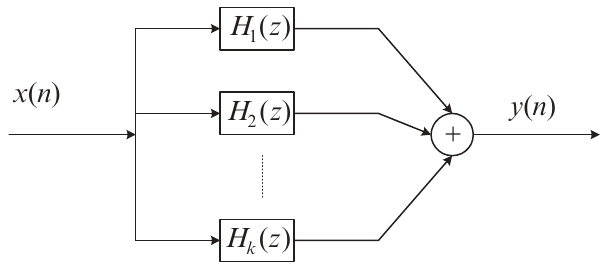
\includegraphics[width=0.8\linewidth]{./img/img06.png}
  \end{figure}
\end{frame}

\begin{frame}{Parallel Realization}
  \textbf{Example:}
  \begin{itemize}
    \item Given a second-order transfer function $$ H(z) = \frac{0.5(1-z^{-2})}{1 + 1.3z^{-1} + 0.36 z^{-2}} $$ perform the filter realizations and write difference equations using Parallel form via first-order sections
  \end{itemize}
\end{frame}

\end{document}